\documentclass[12pt]{article}
\usepackage{epsfig}
\usepackage{natbib}
\usepackage{color}
\usepackage{graphicx}
\usepackage{amssymb,amsmath}

\definecolor{orange}{cmyk}{0,0.4,0.8,0.2}
\definecolor{darkorange}{rgb}{.71,0.21,0.01}
\definecolor{darkgreen}{rgb}{.12,.54,.11}
\definecolor{darkblue}{rgb}{0.1,0.1,0.8}
\definecolor{red}{rgb}{1.0,0,0}
\usepackage{hyperref}
\hypersetup{pdftex,  % needed for pdflatex
  breaklinks=true,  % so long urls are correctly broken across lines
  colorlinks=true,
  urlcolor=blue,
  linkcolor=darkorange,
  citecolor=darkgreen,
  }

\pagestyle{plain}
\topmargin 0in
\headheight 0in
\headsep 0in
\footskip 0.5in

\textheight 9.0in
%\textwidth 6.7in
\textwidth 6.5in

\oddsidemargin 0in
\evensidemargin 0in
\marginparwidth 0in
\baselineskip0.2cm
\parskip0.1cm
\font\cap=cmcsc10

\def\ni{\noindent}        %No Indent%
\def\ub{\underbar}
\def\hi{\noindent \hangindent=2.5em}
\def\et{{\it et\thinspace al.}}    %et al.%
\def\hour{^{\rm h}}
\def\minute{^{\rm m}}
\def\second{^{\rm s}}
\def\arcmin{^{\prime}}
\def\arcsec{^{\prime\prime}}
\def\pixel{{\rm\,pixel}}
\def\degrees{{\rm\,degrees}}
\def\pc{{\rm\,pc}}
\def\cm{{\rm\,cm}}
\def\kms{{\rm\,km/s}}
\def\kpc{{\rm\,kpc}}
\def\hkpc{{\rm\,$h_{50}^{-1}$\,kpc}}
\def\hpc{{\rm\,$h_{50}^{-1}$\,pc}}
\def\Mpc{{\rm\,Mpc}}
\def\mpc{{\rm\,Mpc}}
\def\Gyr{{\rm\,Gyr}}
\def\kmsec{{\rm\,km/s}}
\def\hnot{{\rm\,km/s/Mpc}}
\def\msun{{\rm\,M_\odot}}
\def\lsun{{\rm\,L_\odot}}
\def\mdot{{\rm\,M_\odot}}
\def\surfb{{\rm\,mag/arcsec^2}}
\def\araa{{\it Ann.\ Rev.\ Astr.\ Ap.}}
\def\actaa{{\it Acta~Astronomica}}
\def\aj{{\it A.~J.}}  %Astronomical Journal%
\def\apj{{\it Ap.~J.}}  %Astrophysical Journal%
\def\apjs{{\it Ap.~J.~Suppl.}}  %Astrophysical Journal Supplements%
\def\apjl{{\it Ap.~J.~(Letters)}} %Astrophysical Journal Letters%
\def\pasa{{\it Pub.~A.S.A.}}  %Publications of the Astronomical Society of Australia
\def\pasp{{\it Pub.~A.S.P.}}      %Publications of the Astronomical%
                                %Society of the Pacific%
\def\memsai{{\it Memorie della Societ� Astronomica Italiana}}
\def\mn{{\it M.N.R.A.S.}}      %Monthly Notices of the Royal%
                                %Astronomical Society%
\def\mnras{{\it M.N.R.A.S.}}      %Monthly Notices of the Royal%
                                %Astronomical Society%
\def\nat{{\it Nature}}      %Nature%
\def\aa{{\it Astr.~Ap.}}     %Astronomy & Astrophysics%
\def\aap{{\it Astr.~Ap.}}     %Astronomy & Astrophysics%
\def\aasup{{\it Astr.~Ap.~Suppl.}}     %A & A Supplements%
\def\aaps{{\it Astr.~Ap.~Suppl.}}     %A & A Supplements%
\def\ass{{\it Astr.~Sp.~Sci.}}     %A & A Supplements%
\def\ssr{{\it Space Sci. Rev.}}   %Space Science Reviews%
\def\an{Astronomische~Nachrichten}%
\def\MW{Milky Way }

%
% \lta and \gta produce > and < signs with twiddle underneath
%
\def\spose#1{\hbox to 0pt{#1\hss}}
\def\lta{\mathrel{\spose{\lower 3pt\hbox{$\mathchar"218$}}
     \raise 2.0pt\hbox{$\mathchar"13C$}}}
\def\gta{\mathrel{\spose{\lower 3pt\hbox{$\mathchar"218$}}
     \raise 2.0pt\hbox{$\mathchar"13E$}}}

% also mine!
\def\gsim{\,\lower3pt\hbox{$\sim$}\llap{\raise2pt\hbox{$>$}}\,}
\def\lsim{\,\lower3pt\hbox{$\sim$}\llap{\raise2pt\hbox{$<$}}\,}

% marina
\newcommand{\beqas}{\begin{eqnarray*}}
\newcommand{\eeqas}{\end{eqnarray*}}
\newcommand{\beqa}{\begin{eqnarray}}
\newcommand{\eeqa}{\end{eqnarray}}
\newcommand{\xdelta}{\ensuremath{x^\Delta}}
\newcommand{\comment}[1]{}

\def\xdeltax#1{\ensuremath{x^{\Delta #1}}}
\def\Lo{\hbox{$L_{\odot}$}}
\def\Mo{\hbox{$M_{\odot}$}}

\newcommand{\epss}{\ensuremath{\varepsilon}}
\newcommand{\epsz}{\ensuremath{\varepsilon^0}}
\newcommand{\epstild}{\ensuremath{\tilde{\varepsilon}}}
\newcommand{\psf}{\ensuremath{P\!S\!F\!}}
\newcommand{\SN}{S\!N}
\newcommand{\VS}{V\!S}
\newcommand{\KBO}{K\!B\!O\!}

\newlength{\boxwidth}
\newlength{\boxdown}
\newlength{\boxheight}

\renewcommand{\contentsname}{Table of Contents}

\begin{document}

\title{Deriving Observational Constraints on the Milky Way's Disk using AGB Stars}
\author{Nicholas Hunt-Walker}
\maketitle

% Table of Contents:
\setcounter{page}{0}
\tableofcontents
\vfill
\break

% Body of Proposal
\setcounter{page}{1}
\addcontentsline{toc}{part}{\hspace{1em}Main Science Drivers and Objectives}
\section{Introduction}
The formation of galaxies like the Milky Way was long thought to be a steady process that created a smooth distribution of stars. This standard view was exemplified by the \cite{1980ApJS...44...73B} and \cite{1989ARA&A..27..555G} models, and described in detail by, e.g., \cite{1993ARA&A..31..575M}. In these, the Milky Way is modeled by three discrete components described by simple analytic expressions: the thin disk, thick disk, and halo. Recent discoveries of complex substructure in the distribution of the Milky Way's stars \citep[e.g.][]{2000AJ....120..963I,2000ApJ...540..825Y,2001ApJ...554L..33V,2002ApJ...569..245N,2003ApJ...599.1082M,2006ApJ...642L.137B,2006ApJ...651L..29G,2006AJ....132..714V,2008ApJ...673..864J} have deeply shaken this standard view with indications of signs of rich substructure within the Milky Way Galaxy. This was due to the ability to map the Milky Way using the distances and positions of its own stellar residents. I propose to expand the mapping of the Milky Way, using the ubiquitous stars of the Asymptotic Giant Branch (hereon AGB) as probes to its spatial and chemical structure.

\subsection{First Steps Toward Milky Way Tomography}
Until recently, our knowledge of the basic structural components of the Milky Way was limited to indirect inferences based on stellar population models motivated by other galaxies, and what little information was available from the \emph{High Precision Parallax Collecting Satellite} \cite[HIPPARCOS;][]{1984SSRv...39....1K} catalog and smaller pencil-beam surveys.  The advent of the \emph{Sloan Digital Sky Survey} \citep[SDSS;][]{2000AJ....120.1579Y} alleviated this limitation, providing accurate digital multi-band optical photometry across a quarter of the sky, as well as the largest optical spectroscopic catalog thus far known. SDSS photometry enabled the development and application of photometric parallax methods, using color-magnitude relations to estimate stellar distances. In turn, this led to the large-scale ``tomography" of the Milky Way via stellar distributions in the 7-dimensional space spanned by spatial coordinates \citep{2008ApJ...673..864J}, velocity components \citep{2010ApJ...716....1B}, and metallicity \citep{2008ApJ...684..287I}. The resulting maps provided a quantitative basis for analysis of the main structural components of the Galaxy, enabled efficient searches for complex substructure, and a robust comparison with various model predictions \citep{2012ApJ...757..166B,2012ARA&A..50..251I}.  Figure 1 shows an example of a panoramic view of the variation in the median $[Fe/H]$ over an unprecedentedly-large volume of the Galaxy. %Get this figure and import it here

%-----------
%Fig 1
%\vspace{-10pt}
\begin{figure}[h]
\vspace{-40pt}
\begin{minipage}{0.9\textwidth}
\vbox{
      \begin{minipage}[l]{3in}

     \caption{{\footnotesize
        Median photometric stellar metallicity in cylindrical Galactic coordinates 
        $R$ and $|Z|$  for $\sim$2.5 million stars from SDSS with $14.5 < r <20$,
        $0.2 < g-r < 0.4$, and photometric distance in the 0.8-9 kpc 
        range. %\citep[details in][]{2008ApJ...684..287I}. 
	The gradient of the median metallicity is essentially 
        parallel to the $|Z|$ axis, except in the Monoceros stream. The three squares outline 
        the regions used to measure the 3-dimensional
        velocity distribution for halo stars. The arrows illustrate the variation of the velocity
        ellipsoid orientation, which always points toward the Galactic center.
        The gray scale background is the best-fit model for the stellar number density distribution 
         \citep{2008ApJ...673..864J}. \emph{Top right}: the extent of the data 
        volume relative to the rest of Galaxy, superimposed on the Andromeda 
        Galaxy.  Adapted from 
        \cite{2012ARA&A..50..251I}.
}}
     
      \end{minipage}\ \hfill \
      \begin{minipage}[r]{3in}
	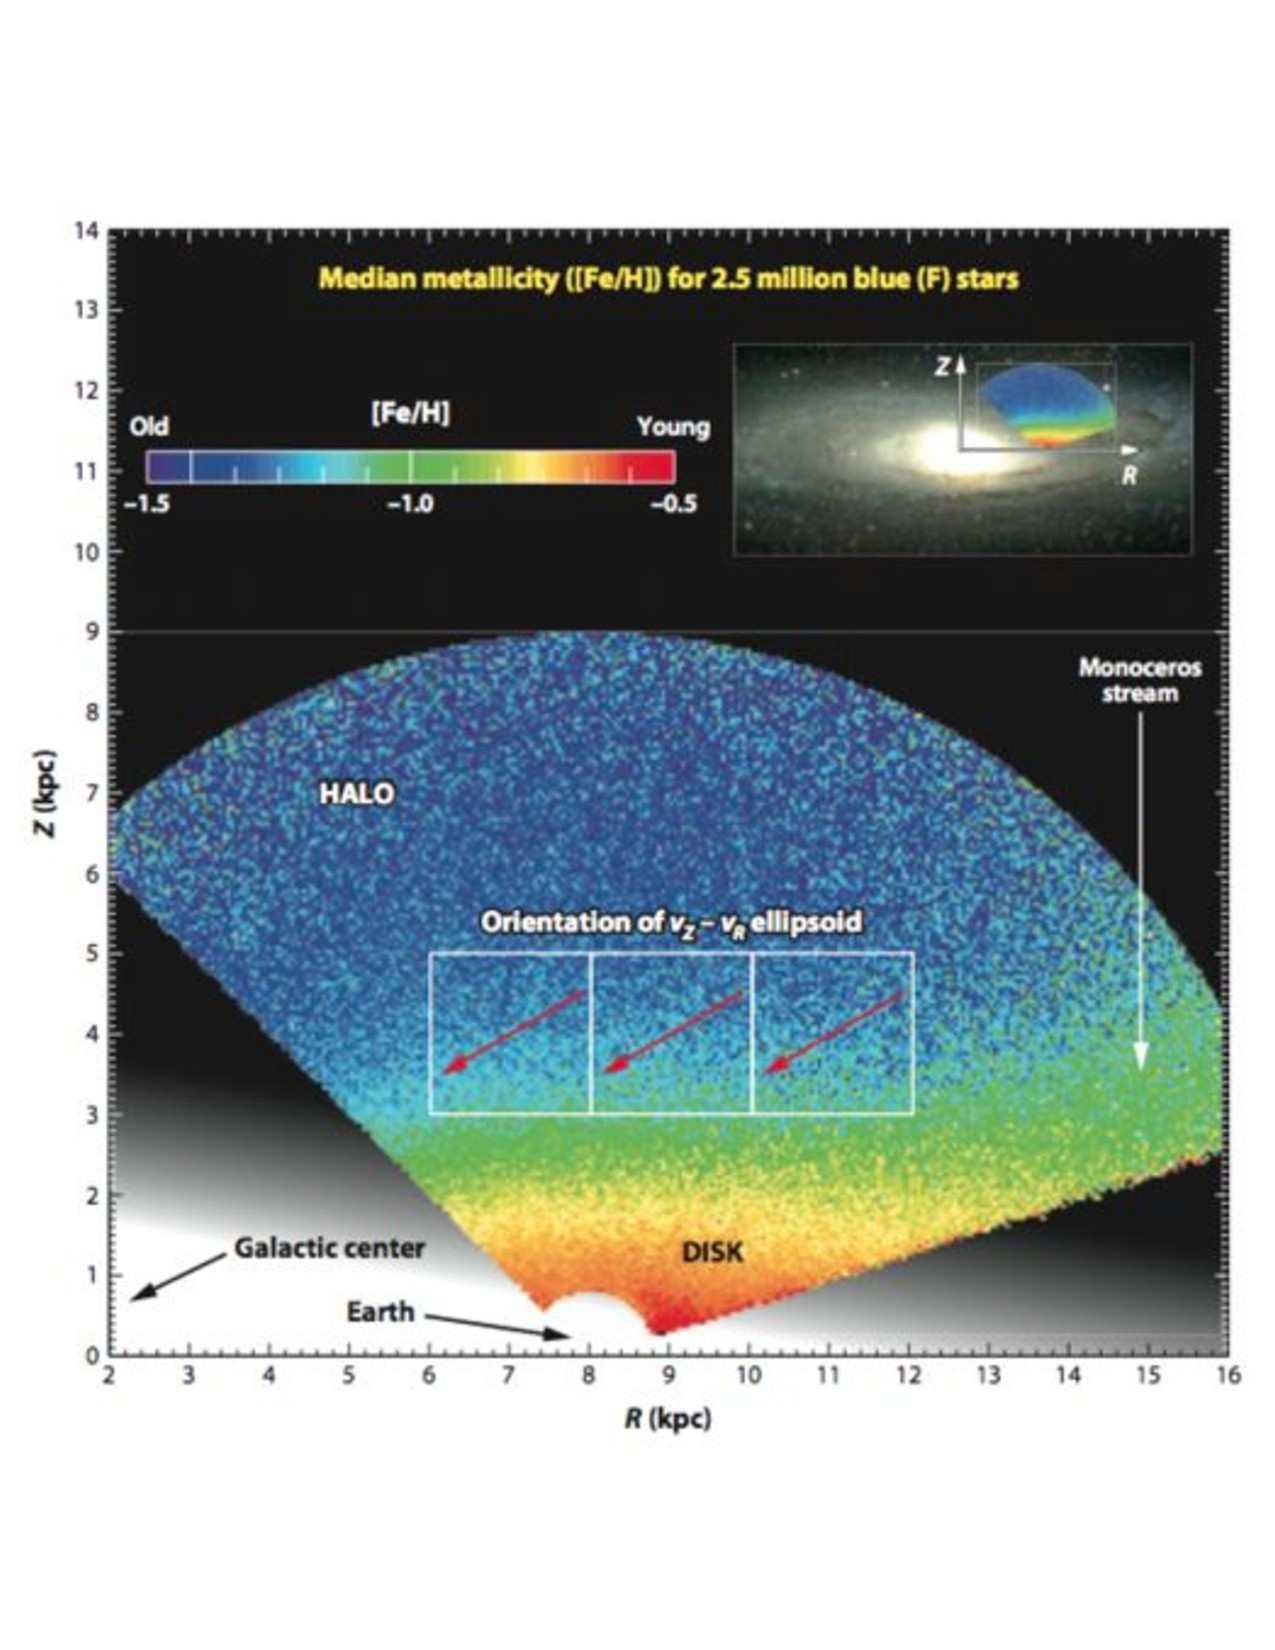
\includegraphics[height=4.5in]{figs/IBJ_fig5.pdf}
%        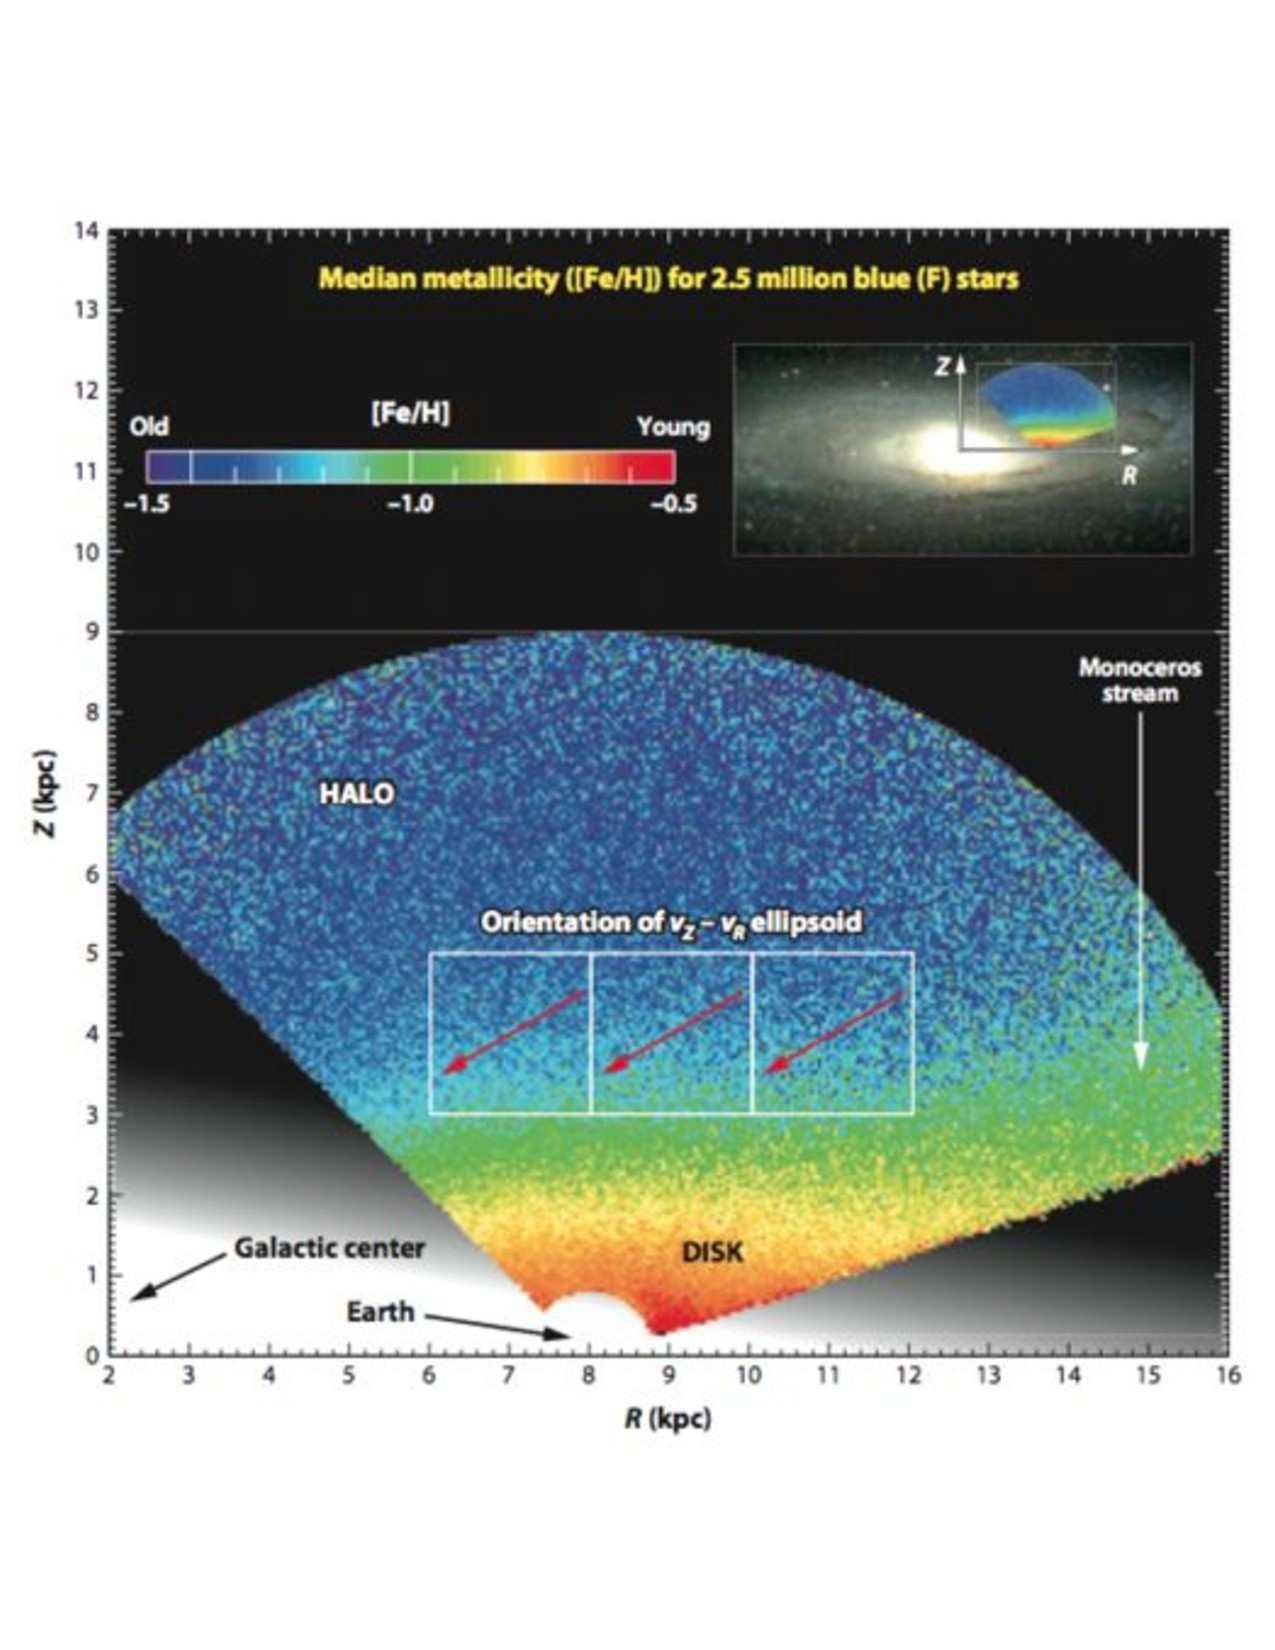
\epsfig{file=figs/IBJ_fig5.pdf, height=4.5in}

      \end{minipage} \ \hfill \
}
\end{minipage}
\vspace{-40pt}
\end{figure}

%------------

\section{Work In Progress/Completed}
\label{sec:completedWork}
The coverage of SDSS in the plane of the Galaxy, and even in the Galactic halo, is thus far limited to the regions targeted by the \emph{Sloan Extension for Galactic Understanding and Exploration} \citep[SEGUE;][]{2012ApJ...757..166B}. More detailed studies of Galactic structure need to rely on the extensive observational capabilities of surveys of the entire sky, using instruments with weak sensitivity to dust extinction. The all-sky survey conducted by the \emph{Wide-field Infrared Survey Explorer} \citep[WISE;][]{2010AJ....140.1868W, 2012wise.rept....1C} gives us the advantage of being able to observe the whole sky in the infrared (IR) at 3.4, 4.6, 12, and 22$\mu$m with unprecedented depth and resolution. The near- and mid-IR (hereon NIR and MIR) are not immune to dust extinction along the line of sight, but the influence of dust on observations is minimal as compared to optical wavelengths \citep{2012ApJ...757..166B, 2014MNRAS.440.3430D}. 

While observations in the NIR and MIR allow us to minimize the influence of dust extinction, and  WISE (particularly the latest data products released as ALLWISE) provides access to the entire sky, a proper survey of the Galaxy requires reliable objects that can be observed throughout the entirety of the Milky Way. AGB stars are the perfect objects to serve as those probes of the Galaxy. AGB stars with dusty circumstellar shells shine brightly in the MIR, particularly with the SiO present in the shells of O-rich stars and the amorphous carbon in shells of C-rich stars \citep{2011A&A...534A..79I}. They are bright enough to be detected by ALLWISE not only near the Galactic center (even with dust extinction), but beyond out to the far edge of the Galactic disk \citep{2013RAA....13..323T}. They're also ubiquitous throughout the Galaxy, being the evolutionary products of 0.8-8 $M_\odot$ Main Sequence stars \citep{1983ARA&A..21..271I}. As such, our work here is first to obtain a clean, reliable sample of these stars within the Galaxy. Once obtained, we can then use the sample of ALLWISE AGB candidates in conjunction with high-confidence models of the Galaxy and of the consequences of AGB star evolution to describe the Milky Way in detail, parameterized by the physical characteristics of AGB stars.

\subsection{Development of Initial Color Criteria for Selecting AGB Stars}
We begin with a known sample of AGB stars, matching them to the ALLWISE-2MASS data release. The MACHO project \citep{2008AJ....136.1242F} and the Optical Gravitational Lens Experiment (OGLE) III Online Catalog of Variable Stars\footnote{\url{http://ogledb.astrouw.edu.pl/~ogle/CVS/}} both contain catalogs of AGB stars, confirmed from their variability. Additionally, the SIMBAD database\footnote{\url{http://simbad.u-strasbg.fr/simbad/}} contains objects classified as AGB stars from small surveys and individual studies. We positionally match these catalogs to objects from the ALLWISE-2MASS data using a circle of uncertainty with radius 1", and necessitate that every match have a 2MASS association.

The region of color-color space occupied by these stars is also occupied by other objects that happen to have dusty environments, as well as naked stars on the main sequence and extragalactic sources. Thus we need a reliable sample of contaminants that we can exclude in color-color space to increase the likelihood that our candidates represent the objects we wish to study. We gather spectroscopically classified AGN, QSOs, and star forming galaxies from the Sloan Digital Sky Survey \citep{2000AJ....120.1579Y} DR 7, specifically the NYU Value-Added Galaxy Catalog\footnote{\url{http://sdss.physics.nyu.edu/vagc/}} \citep[VAGC]{2005AJ....129.2562B}, and LRGs from the SDSS Luminous Red Galaxy Survey \citep{2010ApJ...710.1444K}. Data for stars in the SDSS stellar locus \citep{2014MNRAS.440.3430D} were drawn from the DR 9 SEGUE Stellar Parameters Pipeline (SSPP).

\begin{figure}
% Fig 2
\centering
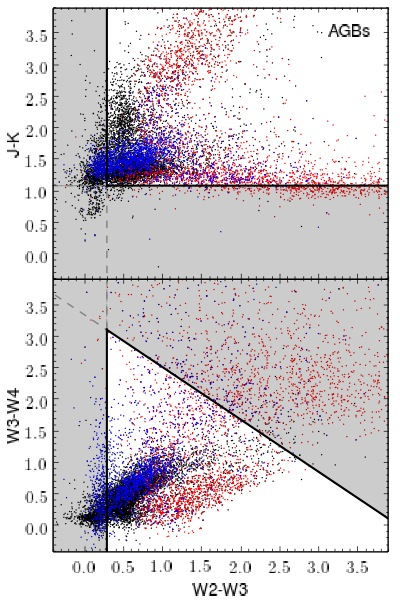
\includegraphics[width=2in]{figs/sampleboundaries.jpg}
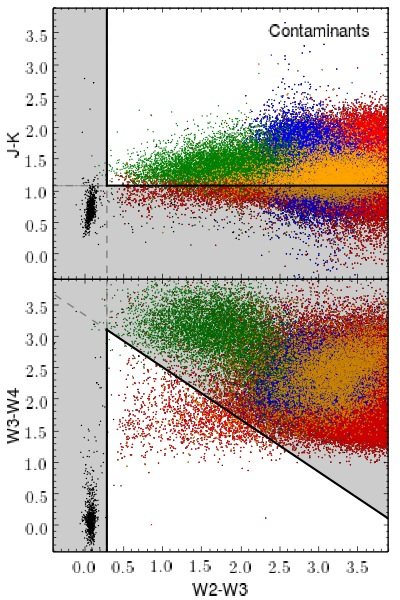
\includegraphics[width=2in]{figs/contamboundaries.jpg}
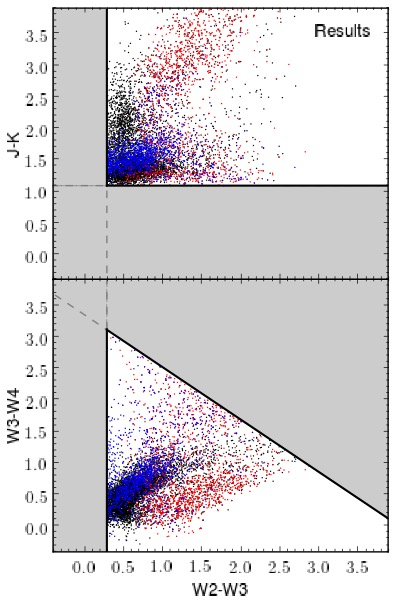
\includegraphics[width=2in]{figs/sample_results.jpg}
\caption{{\footnotesize\emph{Left}: SIMBAD, OGLE-III, and MACHO AGB stars (black, red, blue) matched to ALLWISE within 1". \emph{Middle}: LRGs, starforming galaxies, AGN, QSO, and Locus Stars (green, red, orange, blue, black). \emph{Right}: AGB stars passing ALLWISE color criteria.}}
\label{fig:boundaries}
\end{figure}

The color-color criteria are fairly simple (Figure~\ref{fig:boundaries}): $J-K_s > 1.1$, $W2-W3 > 0.3$, and $W3-W4 < -0.83(W2-W3) + 3.37$. These criteria are set to minimize contamination to  $<1\%$ while retaining as many AGB stars as possible and requiring few cuts in color-color space. We note that in our selection criteria we exclude a substantial population of AGB stars with small or non-existent circumstellar shells. This is necessary in order to also prevent stars from the stellar locus, a far more populous sample, from contaminating our candidates.

\subsection{Estimation of Distances to Candidates with {\tt GALFASTDUST}}
%Create a sample of likely AGB star candidates and use GALFAST to estimate the dust column and distance to each candidate, using the color-color criteria of \cite{2014MNRAS.442.3361N} to differentiate between AGB stars with O-rich and C-rich atmospheres.
\begin{figure}[h]
% Fig 3
\centering
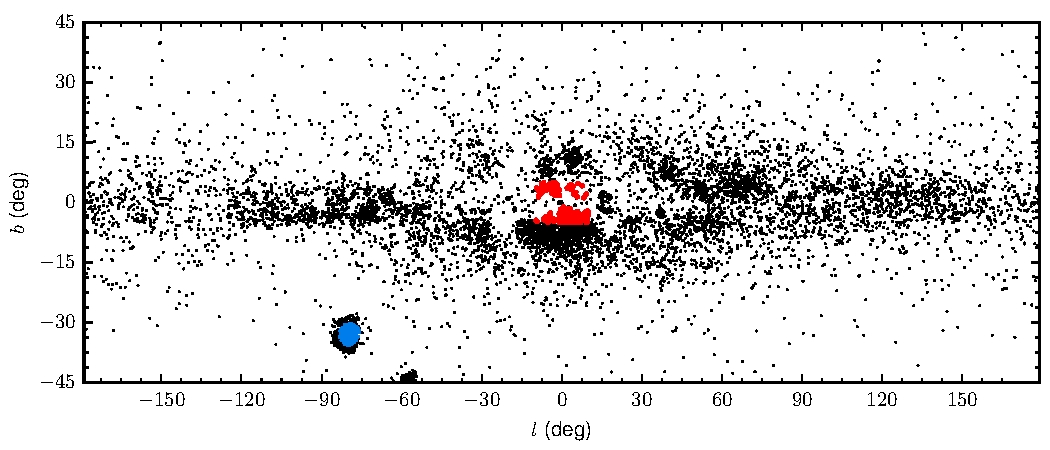
\includegraphics[width=6in]{figs/bulge_lmc_galcoords.pdf}
\caption{{\footnotesize Galactic plot of all AGB stars passing color criteria, highlighting stars in the direction of the bulge (red) and stars in the LMC (blue).}}
\label{fig:galplot}
\end{figure}

As a first step toward creating a 3D map of our Galaxy, we derive reliable color-magnitude relationships for our AGB candidates. From our known sample, we select objects that fit within the narrow color-color criteria for O-rich and C-rich AGB stars set by \cite{2014MNRAS.442.3361N}. We then choose stars in the direction of regions of known distance and high stellar number density: the Milky Way bulge and the Large Magellanic Cloud (red \& blue respectively in Figure~\ref{fig:galplot}). For the LMC, we minimize foreground contamination by selecting stars with $b < -20^\circ$ and also meeting the following criteria:

$$\displaystyle\left(\frac{\text{RA} - \text{RA}_\text{LMC}}{3.5}\right)^2 + \left(\frac{\text{Dec} - \text{Dec}_\text{LMC}}{1.5} \right)^2 < 5 \text{ deg}^2.$$

\noindent With this selection of stars, we demonstrate that AGB stars possess an intrinsically-narrow magnitude distribution, as seen in \cite{1985A&A...152L...1H} and \cite{2002MNRAS.337..749J}. 
%We however do not use this sample further to define the color-magnitude relationships for AGB stars in the IR. The LSST dust extinction code that we use to estimate the dust extinction along the line of sight (hereon {\tt GALFASTDUST}) doesn't include dust in or the shape of the LMC. We neglect to use the Small Magellanic Cloud entirely due to the low object count.  We instead solely use the sample in the direction of the Milky Way bulge for the necessary color-magnitude calibration (Figure~\ref{fig:colormag}). 
We minimize the contamination from foreground stars in the direction of the Galactic bulge by selecting stars with $\lvert l\rvert < 10^\circ$, $1^\circ < \lvert b \rvert < 5^\circ$. 

\begin{figure}[h]
% Fig 4
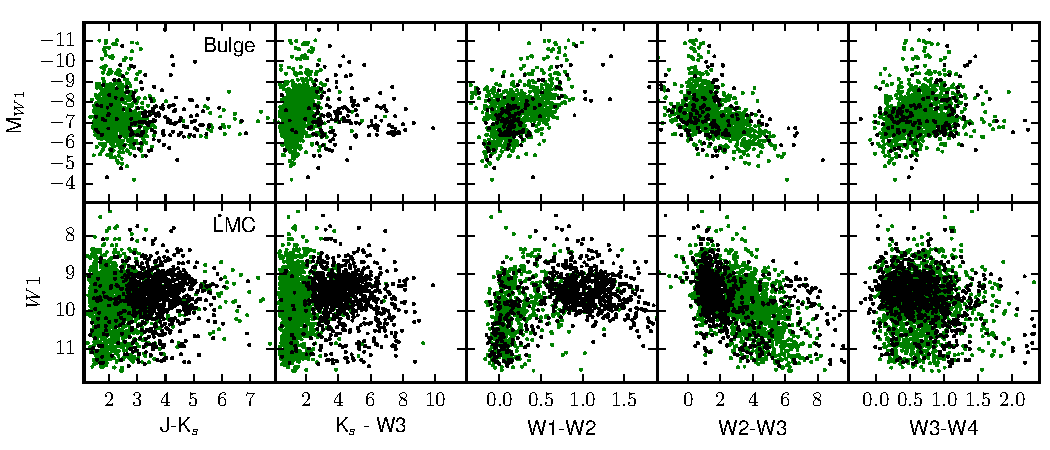
\includegraphics[width=6in]{figs/bulge_lmc_colormag.pdf}
\caption{{\footnotesize Absolute W1 magnitude vs 2MASS-ALLWISE colors for stars in the Milky Way bulge (top) and LMC (bottom). Stars are separated into O-rich (blue) and C-rich (red).}}
\label{fig:colormag}
\end{figure}

Color-magnitude relations are found for each IR color with respect to $M_{w1}$ as derived from the Milky Way bulge using linear regression. With $M_\text{w1}$ calculated with respect to the Milky Way bulge, we use {\tt GALFASTDUST} to simultaneously estimate distance moduli ($DM$) and extinction coefficients ($A_\lambda$) for each object. {\tt GALFASTDUST} returns the color excess $E(B-V)$ for a given ($l$, $b$) and distance $D$ in kpc by placing the object within the axisymmetric galaxy model used by \cite{2005AJ....130..659A}, normalizing $E(B-V)$ to the dust maps of \cite{1998ApJ...500..525S}, and interpolating the dust column along the line of sight. We convert $E(B-V)$ to $A_\lambda$ using the relations in the appendix of \cite{2014MNRAS.440.3430D}. These estimated $DM$ lie within a relatively small degree of uncertainty ($\sim$1 mag), due to scatter about the initial color-magnitude relationship seen in Figure~\ref{fig:colormag}.

Once a candidate sample has been retrieved from the ALLWISE-2MASS database matching our broad color criteria, we narrow them into high-photometric-quality O-rich and C-rich populations using the same criteria from \cite{2014MNRAS.442.3361N}. Assuming absolute magnitudes based upon the aforementioned color-magnitude relationships, we simultaneously estimate the distance and coefficient for dust extinction along the line of sight for each star using {\tt GALFASTDUST}.

\subsection{The Milky Way in 3D and Disk Measurements}
%Create a 3D map of the Galaxy using the aforementioned distances.  Measure the disk scale height as a function of radius, and the disk scale length as a function of height (if possible).
With distance information and position on the sky, we construct an ($X,Y,Z $) map of the Milky Way (Figure~\ref{fig:xyz_candidates}). We note that the overwhelming majority of AGB candidates in the Milky Way are O-rich, with the Galactic population C-rich AGB candidates with high photometric quality being effectively nonexistent, so we move forward solely with an analysis O-rich candidates. We also note, as is clear in Figure~\ref{fig:xyz_candidates}, that this is by no means a complete picture of the Milky Way. The sample is still affected by dust extinction and source confusion, particularly within 0.5 kpc of the Galactic disk, and entirely beyond the bulge within $|b| < 1^\circ$ of the disk. Additionally, because we exclude sources that are beyond the saturation limits of ALLWISE, we lose a large fraction of AGB candidates near the Sun (more toward the Galactic anticenter due to a lack of interstellar dust).

\begin{figure}[h]
% Fig 5
\centering
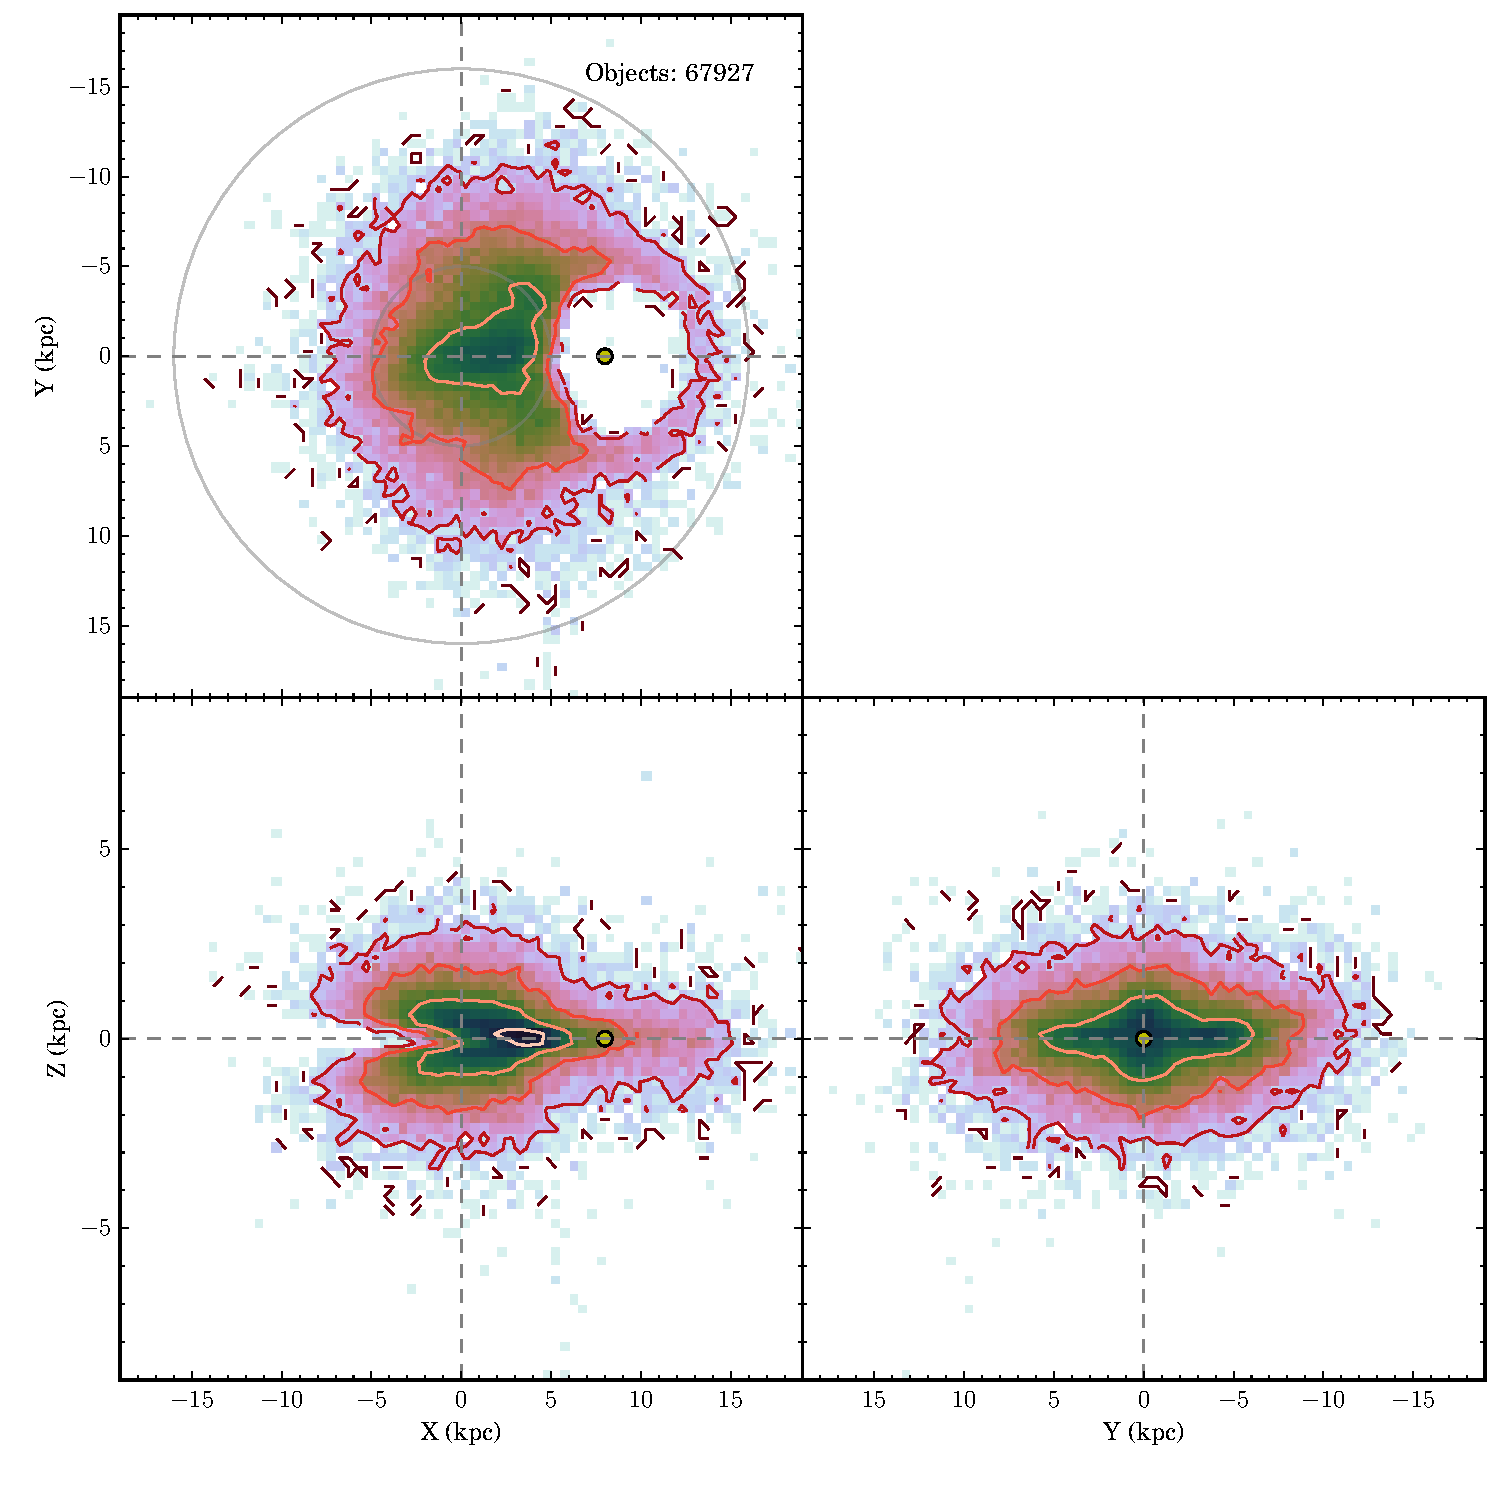
\includegraphics[width=5in]{figs/orich_candidates_xyz.pdf}
\caption{{\footnotesize X-Y-Z distributions of the ALLWISE AGB candidate sample's O-rich stars. The Sun is set as the yellow dot with (X,Y,Z) = (8.0 kpc, 0 kpc, 0 kpc). The gray dashed lines mark (0,0) in each plot, and the contours are spaced by 0.75 logarithmically, starting at 0.}}
\label{fig:xyz_candidates}
\end{figure}

Despite the loss of sources beyond the bulge and near the Sun, we are still able to make measurements of some common disk properties. We focus on the +X half of the Galaxy due to the higher completeness of sources, and exclude the wedge of the Milky Way containing saturation region. We then examine the radial and vertical distribution of AGB candidates, and derive measurements of the scale height as a function of $R$, as well as the scale length as a function of $\lvert Z\rvert$ (Figure~\ref{fig:horvert_profile}).

\begin{figure}[h]
% Fig 6
\centering
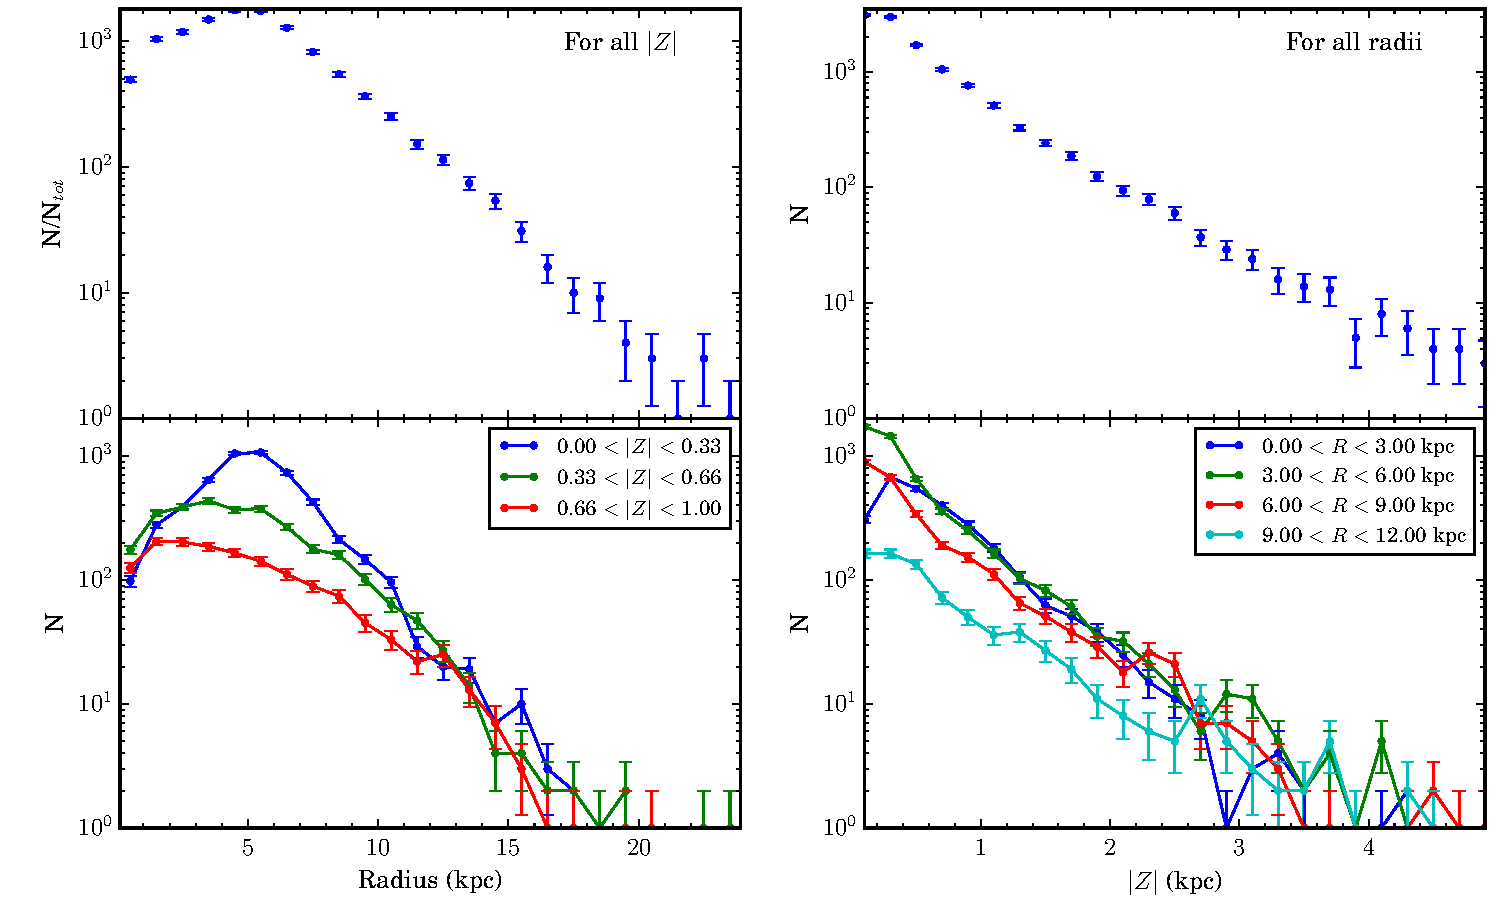
\includegraphics[width=6.5in]{figs/orich_radial_vertical_profile.pdf}
\caption{{\footnotesize Radial (left) and vertical (right) distributions of O-rich AGB candidates in the Milky Way. The top plots show the distributions for all recovered stars, and the bottom plots show the distributions for various heights (left) and radii (right). The radial distributions are in 1 kpc bins, and vertical in 0.2 kpc bins. Uncertainties in each bin are $\sqrt{N}$.}}
\label{fig:horvert_profile}
\end{figure}

\section{Work to be Completed}
The initial groundwork is set for the clean selection of the AGB candidate sample, dust extinction along the line of sight, and distance measurements throughout the Milky Way.  We can proceed to convolve that data with the IR spectroscopic observations from the SDSS \emph{APO Galactic Evolution Experiment} (APOGEE) as well as high quality models of AGB star evolution and Galactic distribution with {\tt TRILEGAL}. We can also investigate those objects not fitting the pre-defined O-rich and C-rich classification schemes.

\subsection{Investigate Unclassified AGB Candidates}
 \cite{2014MNRAS.442.3361N} developed criteria to separate O-rich and C-rich AGB stars based on results from simulations with {\tt DUSTY} \citep{1999astro.ph.10475I}, demonstrating that each population should fall along fairly narrow tracks in WISE color-color space. As previously mentioned, we use these classification schemes to derive color-magnitude relationships for our candidates and produce our Galactic maps. 
 
 However, we can explore wide regions of WISE color-color space and still eliminate the selected contaminants down to the $<$1\% level (Figure~\ref{fig:boundaries}). While this initial effort yields $\sim$215,000 objects qualifying as AGB candidates, the final sample used for mapping the galaxy contained only $\sim$69,000 objects. While many objects may have been lost due to saturation/reliability limits, this still begs the question: what were the other $\sim$150,000 objects, and how did they pass the AGB-trained color-color criteria without explicitly falling in the pre-defined O-rich and C-rich tracks? We seek to answer this by exploring other possible contaminants such as R Cor Borealis stars, young stellar objects, and planetary nebulae \citep{2002MNRAS.337..749J} through positional matches to the SIMBAD database, and verification of AGB candidacy with data from SDSS APOGEE (see section~\ref{sec:apogee}).

\subsection{Comparisons with {\tt TRILEGAL}}
%Same as above, but use TRILEGAL and compare
{\tt TRILEGAL} \citep{2005A&A...436..895G, 2007ASPC..378...20G} provides us with the possibility of testing several quantities produced from the work done thus far. {\tt GALFASTDUST} provided us with an estimation of the dust column along the line of sight to our candidate AGB stars, but with a set Galactic model. {\tt TRILEGAL}  allows us to test the validity of that model, alongside several other models of the Milky Way, with respect to our now-derived 3D distribution of AGB stars by providing stellar number densities along given lines of sight.

With {\tt TRILEGAL}'s simulated photometry, along with various choices of dust chemistry used as input for these simulations, we can use our color-color information as proxies for measurements of photospheric temperature and mass-loss rate, measurements unobtainable from the photometry of ALLWISE. {\tt TRILEGAL} also has the added benefit of producing photometry for any given photometric set. Thus, we would be able to simulate photometry from the GLIMPSE survey, correlate that with photometry from ALLWISE, and use GLIMPSE photometry to fill in the population of AGB stars missing from our current sample due to source confusion and dust extinction. 

Finally, {\tt TRILEGAL} also produces estimations of stellar age, metallicity, [C/O], and periodicity. Convolved with our existing ALLWISE results and potential GLIMPSE results, we may be able to produce a 3D picture of chemical enrichment and age of the Milky Way, while also being able to see the chemical contribution of AGB stars to their local Galactic neighborhoods, giving us an even fuller picture of the evolution of our Galaxy.

\subsection{ALLWISE AGB Candidates and APOGEE}
\label{sec:apogee}
%Match candidate sample to APOGEE red giant survey to get actual stellar parameters as a function of position. Use above relationships to estimate circumstellar shell size, age, mass-loss rate, metallicity, anything really. Correlate that with X-Y-Z position in the Galaxy (or maybe even just R-Z).
The SDSS APOGEE survey observed $1.6\times10^5$ giant stars to $H < 12.2$ with NIR spectroscopy \citep{2012ApJ...755L..25N}. We have matched the ALLWISE AGB candidate sample to the latest results from the APOGEE survey, retrieving $\sim$8,500 objects positionally matching our cleanest sample to within 1", with most positions $0.4"$ apart (Figure~\ref{fig:apogee_allwise}).  This provides us with precise measurements of stellar properties unable to be obtained from ALLWISE that we can now use to characterize our sample, provide measurable checks as to the reliability of our sample, as well as improve upon the existing capabilities and outputs of {\tt TRILEGAL}.

\begin{figure}[h]
% Fig 7
\centering
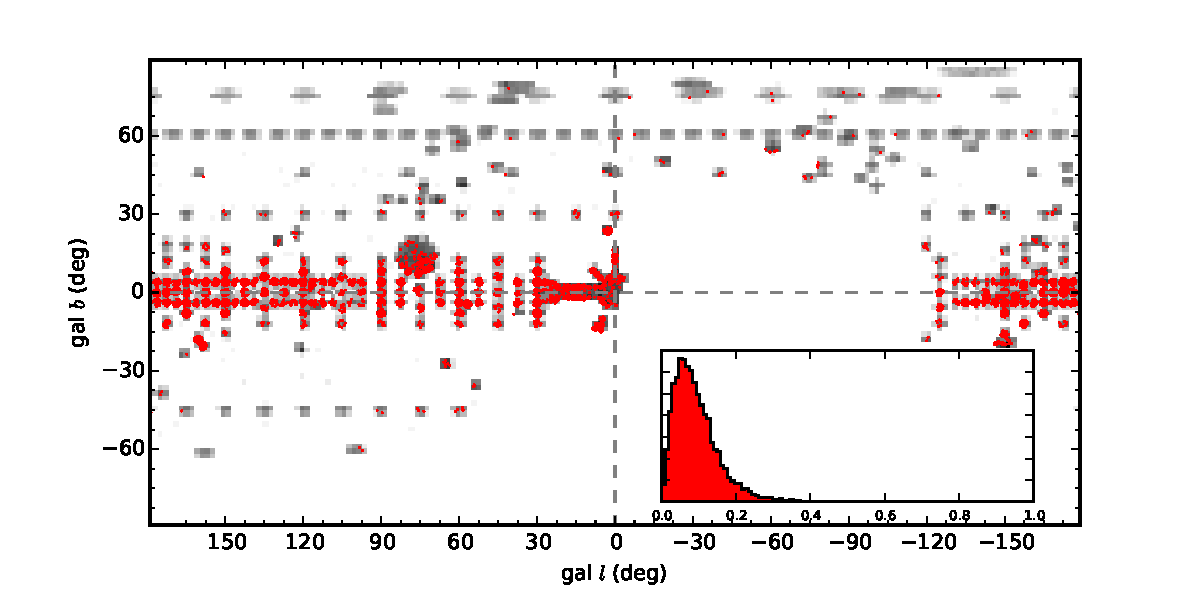
\includegraphics[width=6.5in]{figs/apogee_allwise_overlay.pdf}
\caption{{\footnotesize APOGEE sources (gray) overlaid with matches within 1" from ALLWISE AGB candidates (red). \emph{Inset}: Distribution of matching radii between APOGEE and ALLWISE catalogs out to 1".}}
\label{fig:apogee_allwise}
\end{figure}

With the input from APOGEE, we will correlate various stellar properties (e.g. $T_\text{eff}$, $[Fe/H]$) with ALLWISE-2MASS colors for our AGB candidate sample. ALLWISE-2MASS IR colors, particularly $W2-W3$ and $W3-W4$, are sensitive to the composition and size of the AGB circumstellar shell, making chemical differences separable in ALLWISE color-color space as demonstrated by \cite{2014MNRAS.442.3361N}. We should then be able to use standard machine learning techniques \citep[e.g. those found in ][]{2013sdmm.book.....I} to extend estimates of these same stellar parameters to stars that were not initially matched to APOGEE due to lying outside either the photometric or spatial range of APOGEE.

Comparison of the candidate sample to APOGEE will also provide us with a test against the axisymmetric Galactic model used by {\tt GALFASTDUST}. Obviously the Milky Way is not a simple axisymmetric system, containing large structures such as spiral arms, as well as the various overdensities observed by \cite{2008ApJ...673..864J} and others that have followed.  With measurements from APOGEE we will be able to comment on the accuracy of our previous 3D distribution and improve upon observations of substructure in the Milky Way.

\section{Timeline}
\begin{enumerate}
\item Paper 1: Publication of AGB candidate catalog and preliminary measurements of Milky Way disk and bulge -- \textbf{End of March 2015}
	\begin{itemize}
		\item Sample selection completeness and contamination estimates
		\item O-rich/C-rich classification from color-color criteria
		\item Identification of unclassified candidates
		\item Estimates of unconfirmed classifications with Gaussian Mixture Models
		\item Measurements of disk scale height/length
		\item Measurements of the sizes of the Galactic bar \& bulge and orientation of the Galactic bar
		\item Measurement of radius of Galactic disk
	\end{itemize}	

\item Paper 2: Characteristics of the Milky Way galaxy via ALLWISE AGB candidates -- \textbf{End of Sept 2015}
	\begin{itemize}
		\item Mass-loss rate, model metallicity, temperature, size, and age of AGB candidates with respect to position
		\item Interpretations of position-dependent characteristics
		\item Meaning of these results with respect to improvements in AGB evolutionary tracks
	\end{itemize}
	
\item Post doctorate job applications -- \textbf{Oct-Nov 2015}
\item Paper 3: AGB stellar parameters from APOGEE and extrapolation to entire candidate sample -- \textbf{May 2016}
	\begin{itemize}
		\item Matches between ALLWISE candidates and APOGEE targets
		\item Color-parameter relationships between APOGEE and ALLWISE
		\item Extrapolation to entire candidate sample through color-parameter relationships
		\item Comparison to estimations from various machine-learning techniques
		\item Comparison to estimations from TRILEGAL
	\end{itemize}
\item Dissertation preparation -- \textbf{June - August 2016}
\item Defense -- \textbf{August/September 2016}
\end{enumerate}

\section{Potential Future Work}
This work when completed will be just in time to set the stage for a few ambitious projects, and will be prime for building new and strengthening existing collaborative works.

\subsection{From Candidates to Confirmations}
AGB stars are known for their long-period variability of $\Delta V\sim2.5$ mag on timescales of $\sim$1 year \citep{2000PASA...17...18W, 2008PhDT.........6F}. With accurate time-series photometry these stars can be confirmed without the need for spectroscopy across tens of thousands of sources. A prime candidate for such all-sky time-series data is the European Space Agency's Gaia space observatory \citep{2001A&A...369..339P,2002MNRAS.331..649B}. With unprecedented astrometry and photometric sensitivity in the optical and NIR, as well as between 40 and 250 visits per object over 5 years down to $V$ = 20 mag, it will be trivial for Gaia to identify long period variables in our existing candidate sample \citep{2000ASPC..203...71E}.

\subsection{Investigating the TP-AGB and {\tt COLIBRI}}
The AGB parameters output by version 2.3 of {\tt TRILEGAL} uses the population synthesis code {\tt COLIBRI}, which includes the thermally-pulsing (TP) phase of the AGB \citep{2013MNRAS.434..488M}. This code is calibrated using observations from the Magellanic Clouds, but would benefit greatly from a healthy sample of AGB stars from the Galaxy. APOGEE is already providing $\sim$8,300 of our objects with high-quality spectroscopic measurements, however as seen in Figure~\ref{fig:apogee_allwise} it neglects large portions of the Galaxy. With a large-scale spectroscopic program aimed at precise measurements of characteristics of the remaining AGB stars from this sample, we'd be able to contribute to this ongoing work with a thorough characteriziation of Galactic AGB stars. Specifically, we'd be able to accurately identify populations of TP-AGB stars as well as provide reliable measurements of the C/O ratios with position in the Milky Way alongside our existing IR measurements.






\vfill
\break

% References
\addcontentsline{toc}{part}{\hspace {1em}References}
\bibliographystyle{apj}
\bibliography{thesisproprefs}
\vfill
\eject



\end{document}